\documentclass{standalone}
\usepackage{tikz}
\usetikzlibrary{patterns, positioning}
\usepackage[sfdefault]{ClearSans} %% option 'sfdefault' activates Clear Sans as the default text font
\usepackage[T1]{fontenc}

\begin{document}
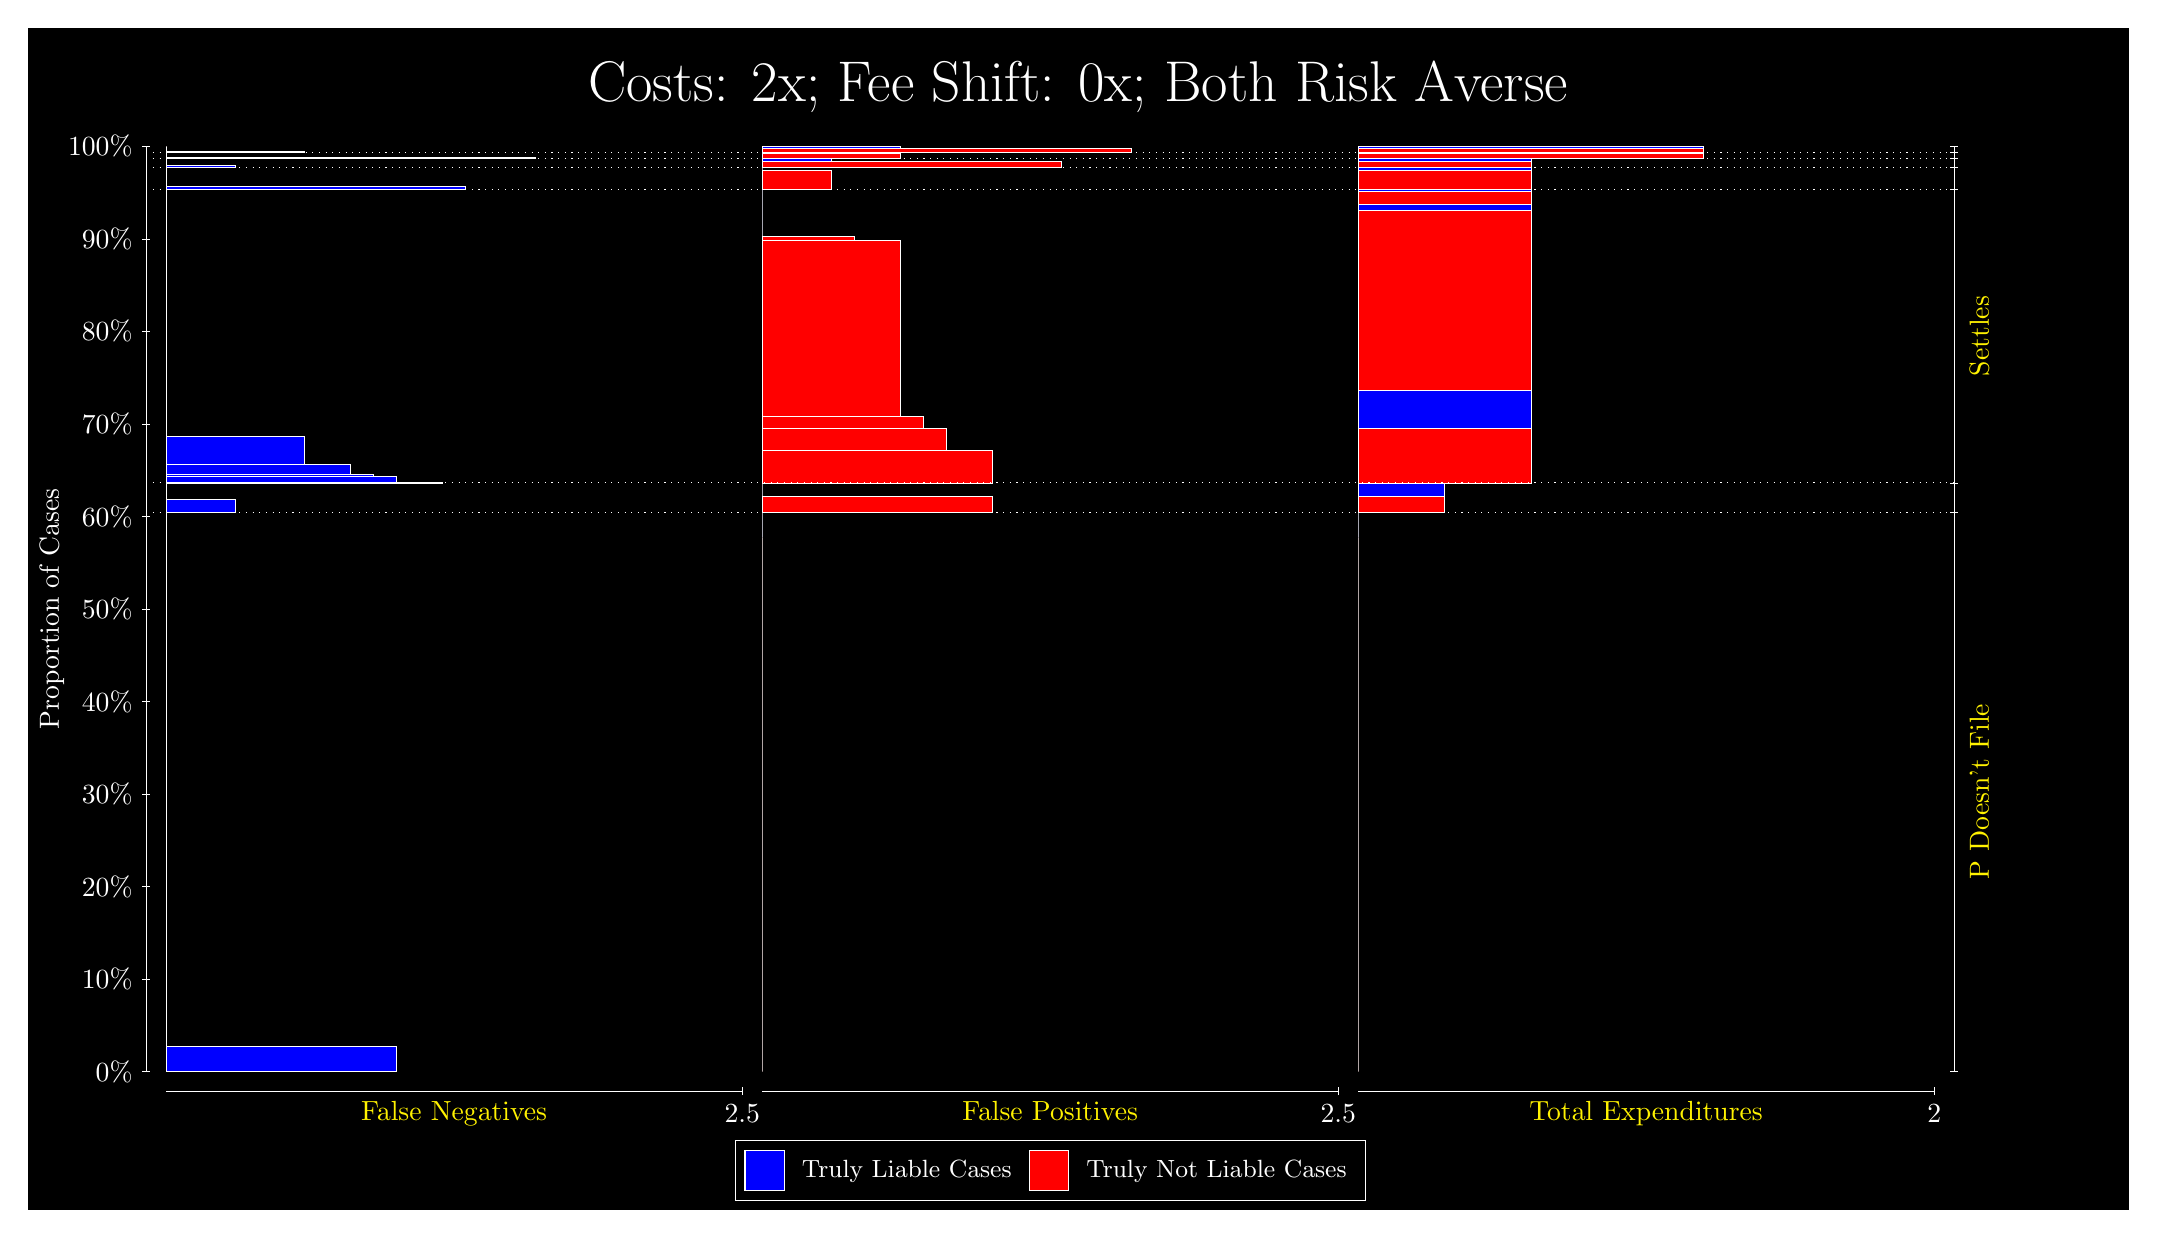
\begin{tikzpicture}
\draw[fill=black] (0,0) rectangle (26.667,15);
\draw[text=white] (0,13.5) rectangle (26.667,15) node[midway] {\huge Costs: 2x; Fee Shift: 0x; Both Risk Averse};
\draw[white, very thin] (1.5,1.75) -- (1.5,13.5);
\node[rotate=90, text=white, anchor=center] at (0.3, 7.625) {Proportion of Cases};
\draw[white, very thin] (1.45,1.75) -- (1.55,1.75);
\node[text=white, anchor=east] at (1.45, 1.75) {0\%};
\draw[white, very thin] (1.45,2.925) -- (1.55,2.925);
\node[text=white, anchor=east] at (1.45, 2.925) {10\%};
\draw[white, very thin] (1.45,4.1) -- (1.55,4.1);
\node[text=white, anchor=east] at (1.45, 4.1) {20\%};
\draw[white, very thin] (1.45,5.275) -- (1.55,5.275);
\node[text=white, anchor=east] at (1.45, 5.275) {30\%};
\draw[white, very thin] (1.45,6.45) -- (1.55,6.45);
\node[text=white, anchor=east] at (1.45, 6.45) {40\%};
\draw[white, very thin] (1.45,7.625) -- (1.55,7.625);
\node[text=white, anchor=east] at (1.45, 7.625) {50\%};
\draw[white, very thin] (1.45,8.8) -- (1.55,8.8);
\node[text=white, anchor=east] at (1.45, 8.8) {60\%};
\draw[white, very thin] (1.45,9.975) -- (1.55,9.975);
\node[text=white, anchor=east] at (1.45, 9.975) {70\%};
\draw[white, very thin] (1.45,11.15) -- (1.55,11.15);
\node[text=white, anchor=east] at (1.45, 11.15) {80\%};
\draw[white, very thin] (1.45,12.325) -- (1.55,12.325);
\node[text=white, anchor=east] at (1.45, 12.325) {90\%};
\draw[white, very thin] (1.45,13.5) -- (1.55,13.5);
\node[text=white, anchor=east] at (1.45, 13.5) {100\%};

\draw[white, very thin] (24.457,1.75) -- (24.457,13.5);
\draw[white, very thin] (24.407,1.75) -- (24.507,1.75);
\node[anchor=west] at (24.407, 1.75) {};
\draw[white, very thin] (24.407,8.8542) -- (24.507,8.8542);
\node[anchor=west] at (24.407, 8.8542) {};
\draw[white, very thin] (24.407,9.2251) -- (24.507,9.2251);
\node[anchor=west] at (24.407, 9.2251) {};
\draw[white, very thin] (24.407,12.956) -- (24.507,12.956);
\node[anchor=west] at (24.407, 12.956) {};
\draw[white, very thin] (24.407,13.23) -- (24.507,13.23);
\node[anchor=west] at (24.407, 13.23) {};
\draw[white, very thin] (24.407,13.349) -- (24.507,13.349);
\node[anchor=west] at (24.407, 13.349) {};
\draw[white, very thin] (24.407,13.419) -- (24.507,13.419);
\node[anchor=west] at (24.407, 13.419) {};
\draw[white, very thin] (24.407,13.5) -- (24.507,13.5);
\node[anchor=west] at (24.407, 13.5) {};

\draw[white, very thin, fill=blue] (1.75,1.75) rectangle (4.6775,2.0695);
\draw[white, very thin, fill=red] (1.75,2.0695) rectangle (1.75,8.8542);
\draw[white, very thin, fill=blue] (1.75,8.8542) rectangle (2.6283,9.0179);
\draw[white, very thin, fill=red] (1.75,9.0179) rectangle (1.75,9.2251);
\draw[white, very thin, fill=blue] (1.75,9.2251) rectangle (5.2631,9.2313);
\draw[white, very thin, fill=blue] (1.75,9.2313) rectangle (4.6775,9.3081);
\draw[white, very thin, fill=blue] (1.75,9.3081) rectangle (4.3848,9.3367);
\draw[white, very thin, fill=blue] (1.75,9.3367) rectangle (4.092,9.4641);
\draw[white, very thin, fill=blue] (1.75,9.4641) rectangle (3.5065,9.8191);
\draw[white, very thin, fill=red] (1.75,9.8191) rectangle (1.75,12.956);
\draw[white, very thin, fill=blue] (1.75,12.956) rectangle (5.5558,12.989);
\draw[white, very thin, fill=red] (1.75,12.989) rectangle (1.75,13.23);
\draw[white, very thin, fill=blue] (1.75,13.23) rectangle (2.6283,13.265);
\draw[white, very thin, fill=red] (1.75,13.265) rectangle (1.75,13.349);
\draw[white, very thin, fill=blue] (1.75,13.349) rectangle (6.4341,13.355);
\draw[white, very thin, fill=red] (1.75,13.355) rectangle (1.75,13.419);
\draw[white, very thin, fill=blue] (1.75,13.419) rectangle (3.5065,13.442);
\draw[white, very thin, fill=red] (1.75,13.442) rectangle (1.75,13.5);
\draw[white, very thin, fill=red] (9.3189,1.75) rectangle (9.3189,8.5347);
\draw[white, very thin, fill=blue] (9.3189,8.5347) rectangle (9.3189,8.8542);
\draw[white, very thin, fill=red] (9.3189,8.8542) rectangle (12.246,9.0614);
\draw[white, very thin, fill=blue] (9.3189,9.0614) rectangle (9.3189,9.2251);
\draw[white, very thin, fill=red] (9.3189,9.2251) rectangle (12.246,9.6398);
\draw[white, very thin, fill=red] (9.3189,9.6398) rectangle (11.661,9.9149);
\draw[white, very thin, fill=red] (9.3189,9.9149) rectangle (11.368,10.076);
\draw[white, very thin, fill=red] (9.3189,10.076) rectangle (11.075,12.307);
\draw[white, very thin, fill=red] (9.3189,12.307) rectangle (10.49,12.362);
\draw[white, very thin, fill=blue] (9.3189,12.362) rectangle (9.3189,12.956);
\draw[white, very thin, fill=red] (9.3189,12.956) rectangle (10.197,13.197);
\draw[white, very thin, fill=blue] (9.3189,13.197) rectangle (9.3189,13.23);
\draw[white, very thin, fill=red] (9.3189,13.23) rectangle (13.125,13.313);
\draw[white, very thin, fill=blue] (9.3189,13.313) rectangle (10.197,13.349);
\draw[white, very thin, fill=red] (9.3189,13.349) rectangle (11.075,13.412);
\draw[white, very thin, fill=blue] (9.3189,13.412) rectangle (9.3189,13.419);
\draw[white, very thin, fill=red] (9.3189,13.419) rectangle (14.003,13.477);
\draw[white, very thin, fill=blue] (9.3189,13.477) rectangle (11.075,13.5);
\draw[white, very thin, fill=red] (16.888,1.75) rectangle (16.888,8.5347);
\draw[white, very thin, fill=blue] (16.888,8.5347) rectangle (16.888,8.8542);
\draw[white, very thin, fill=red] (16.888,8.8542) rectangle (17.986,9.0614);
\draw[white, very thin, fill=blue] (16.888,9.0614) rectangle (17.986,9.2251);
\draw[white, very thin, fill=red] (16.888,9.2251) rectangle (19.083,9.9149);
\draw[white, very thin, fill=blue] (16.888,9.9149) rectangle (19.083,10.397);
\draw[white, very thin, fill=red] (16.888,10.397) rectangle (19.083,12.684);
\draw[white, very thin, fill=blue] (16.888,12.684) rectangle (19.083,12.767);
\draw[white, very thin, fill=red] (16.888,12.767) rectangle (19.083,12.928);
\draw[white, very thin, fill=blue] (16.888,12.928) rectangle (19.083,12.956);
\draw[white, very thin, fill=red] (16.888,12.956) rectangle (19.083,13.197);
\draw[white, very thin, fill=blue] (16.888,13.197) rectangle (19.083,13.23);
\draw[white, very thin, fill=red] (16.888,13.23) rectangle (19.083,13.313);
\draw[white, very thin, fill=blue] (16.888,13.313) rectangle (19.083,13.349);
\draw[white, very thin, fill=red] (16.888,13.349) rectangle (21.279,13.412);
\draw[white, very thin, fill=blue] (16.888,13.412) rectangle (21.279,13.419);
\draw[white, very thin, fill=red] (16.888,13.419) rectangle (21.279,13.477);
\draw[white, very thin, fill=blue] (16.888,13.477) rectangle (21.279,13.5);
\draw[white, dotted] (1.5,8.8542) -- (24.457,8.8542);
\draw[white, dotted] (1.5,9.2251) -- (24.457,9.2251);
\draw[white, dotted] (1.5,12.956) -- (24.457,12.956);
\draw[white, dotted] (1.5,13.23) -- (24.457,13.23);
\draw[white, dotted] (1.5,13.349) -- (24.457,13.349);
\draw[white, dotted] (1.5,13.419) -- (24.457,13.419);
\draw[white, very thin] (1.75,1.5) -- (9.0689,1.5);
\node[text=yellow, anchor=north] at (5.4094, 1.5) {False Negatives};
\draw[white, very thin] (9.0689,1.45) -- (9.0689,1.55);
\node[text=white, anchor=north] at (9.0689, 1.45) {2.5};

\draw[white, very thin] (9.3189,1.5) -- (16.638,1.5);
\node[text=yellow, anchor=north] at (12.978, 1.5) {False Positives};
\draw[white, very thin] (16.638,1.45) -- (16.638,1.55);
\node[text=white, anchor=north] at (16.638, 1.45) {2.5};

\draw[white, very thin] (16.888,1.5) -- (24.207,1.5);
\node[text=yellow, anchor=north] at (20.547, 1.5) {Total Expenditures};
\draw[white, very thin] (24.207,1.45) -- (24.207,1.55);
\node[text=white, anchor=north] at (24.207, 1.45) {2};

\node[text=yellow, centered, rotate=90] at (24.777, 5.3021) {P Doesn't File};

\node[text=yellow, centered, rotate=90] at (24.777, 11.091) {Settles};





\draw (12.978300999999998,1.5) node[draw=none] (baseCoordinate) {};
\begin{scope}[align=center]
        \matrix[scale=0.5, draw=white, below=0.5cm of baseCoordinate, nodes={draw}, column sep=0.1cm]{
            \node[rectangle, draw, minimum width=0.5cm, minimum height=0.5cm, fill=blue] {}; &
            \node[draw=none, font=\small, text=white] (B) {Truly Liable Cases}; &
            \node[rectangle, draw, minimum width=0.5cm, minimum height=0.5cm, fill=red] {}; &
            \node[draw=none, font=\small, text=white] (B) {Truly Not Liable Cases}; \\
            };
\end{scope}

\end{tikzpicture}
\end{document}